\section{Iteratori}
Un iteratore è una struttura dati dotata di stato, in grado di generare una sequenza di valori.
I valori possono essere estratti da un contenitore, di cui l'iteratore detiene un riferimento, o generati programmaticamente, come nel caso di un intervallo di valori.

Un iteratore offre tipicamente un modo per verificare se sono presenti ulteriori valori da generare (\mintinline{rust}|hasNext() -> bool|) ed un altro per accedere al valore successivo (\mintinline{rust}|next() -> E|).
Talora, come in Rust, le due operazioni sono combinate (\mintinline{rust}|next() -> Option<E>|).
Inoltre, un iteratore può offrire ulteriori metodi che consentono di derivare un nuovo iteratore, che trasforma la sequenza di valori in un'altra sequenza (accorpando, eliminando, trasformando, ecc., i singoli elementi originali).

Pressoché tutti i linguaggi "moderni" offrono il concetto di iteratore come parte della propria libreria standard.
Essi permettono di accedere ai valori contenuti all'interno di collezioni come liste, insiemi, mappe, scorrere i caratteri presenti all'interno di una stringa o leggere il contenuto di un file di testo estraendo una riga alla volta.

\subsection{Uso degli iteratori}
L'uso degli iteratori si sovrappone concettualmente a quello dei cicli \verb|for|/\verb|while|.
Tuttavia, offre svariati vantaggi in termini di compattezza del codice, leggibilità, manutenibilità ed efficienza, nascondendo i dettagli necessari a generare o accedere ai singoli elementi.
I vantaggi sono maggiormente evidenti se l'operazione svolta all'interno del ciclo è complessa e richiede, ad esempio, di scartare alcuni valori e di trasformarne altri.

\begin{center}
  \begin{minipage}{0.48\linewidth}
    \begin{tcolorbox}[title=Approccio Imperativo]
      \begin{minted}[breaklines]{rust}
let v1 = vec![1, 2, 3, 4, 5, 6]; 
let mut v2 = Vec::<String>::new(); 
for i in 0..v1.len() { 
    if v1[i] % 2 != 0 { continue; } 
    v2.push(format!("a{}", v1[i])) 
} 
println!("{:?}", v2); 
// ["a2", "a4", "a6"]
        \end{minted}
    \end{tcolorbox}
  \end{minipage}%
  \hfill
  \begin{minipage}{0.48\linewidth}
    \begin{tcolorbox}[title=Approccio Funzionale (Iteratori)]
      \begin{minted}[breaklines]{rust}
let v1 = vec![1, 2, 3, 4, 5, 6]; 
let mut v2: Vec<String>; 
v2 = v1.iter() 
    .filter(|val| { *val % 2 == 0 }) 
    .map(|val| format!("a{}", val)) 
    .collect(); 
println!("{:?}", v2); 
// ["a2", "a4", "a6"]
        \end{minted}
    \end{tcolorbox}
  \end{minipage}
\end{center}

\subsection{Caratteristiche degli iteratori}
\begin{itemize}
  \item Un iteratore offre un modo uniforme di accedere agli elementi, indipendentemente da come essi siano generati o da dove siano prelevati, permettendo al codice che utilizza tali valori di ignorare la fonte ed essere più generico.
  \item Gli iteratori operano in \textbf{modalità pigra (lazy)}: solo a fronte della richiesta di un valore successivo, si occupano di generarlo / prelevarlo.
  \item Possono abilitare l'elaborazione parallela dei dati ospitati in una collezione, permettendo di sfruttare la presenza di più core nell'elaboratore.
  \item La possibilità di derivare un iteratore da un altro iteratore aumenta la flessibilità del codice. È facile inserire all'interno di una catena di elaborazione passi ulteriori senza dover intervenire sul codice che utilizza i valori generati.
\end{itemize}

\section{Iteratori in Rust}
In Rust, un iteratore è una qualsiasi struttura dati che implementa il tratto \verb|std::iter::Iterator|.
Un tipo può segnalare la capacità di essere esplorato tramite un iteratore, implementando il tratto \verb|std::iter::IntoIterator|.

\begin{minted}[breaklines]{rust}
trait Iterator { 
    type Item; 
    fn next(&mut self) -> Option<Self::Item>;    // ... molti altri metodi con implementazione di default
} 

trait IntoIterator where Self::IntoIter: Iterator<Item=Self::Item> { 
    type Item; 
    type IntoIter: Iterator; 
    fn into_iter(self) -> Self::IntoIter; 
} 
\end{minted}

\subsection{Implementare un iteratore in Rust}
Esempio di implementazione di un iteratore per un range di valori personalizzato:

\begin{minted}[breaklines]{rust}
struct MyRange<const FROM: isize, const TO: isize> {} 

impl<const FROM: isize, const TO: isize> IntoIterator for MyRange<FROM, TO> { 
    type Item = isize; 
    type IntoIter = MyRangeIterator<FROM, TO>; 
    fn into_iter(self) -> Self::IntoIter { 
        MyRangeIterator::<FROM, TO>::new() 
    } 
} 

struct MyRangeIterator<const FROM: isize, const TO: isize> { val: isize } 

impl<const FROM: isize, const TO: isize> MyRangeIterator<FROM, TO> { 
    fn new() -> Self { 
        MyRangeIterator { val: FROM } 
    } 
} 

impl<const FROM: isize, const TO: isize> Iterator for MyRangeIterator<FROM, TO> { 
    type Item = isize; 
    fn next(&mut self) -> Option<Self::Item> { 
        if FROM < TO { 
            if self.val < TO { 
                let ret = self.val; 
                self.val += 1; 
                Some(ret) 
            } else { None } 
        } else { 
            if self.val > TO { 
                let ret = self.val; 
                self.val -= 1; 
                Some(ret) 
            } else { None } 
        } 
    } 
} 
\end{minted}

\section{Iteratori e possesso}
I contenitori presenti nella libreria standard mettono normalmente a disposizione tre metodi per ricavare un iteratore ai dati contenuti al loro interno:

\begin{itemize}
  \item \mintinline{rust}|iter()|: restituisce oggetti di tipo \mintinline{rust}|&Item| e non consuma il contenuto del contenitore.
  \item \mintinline{rust}|iter_mut()|: restituisce oggetti di tipo \mintinline{rust}|&mut Item| e permette di modificare gli elementi all'interno del contenitore.
  \item \mintinline{rust}|into_iter()|: prende possesso del contenitore e restituisce oggetti di tipo \mintinline{rust}|Item| estraendoli dal contenitore.
\end{itemize}

È comune, per tali contenitori, dichiarare tre implementazioni distinte del tratto \verb|IntoIterator|: una per il tipo \verb|Container| (\mintinline{rust}|into_iter()|), una per il tipo \verb|&Container| (\mintinline{rust}|iter()|), e una per il tipo \verb|&mut Container| (\mintinline{rust}|iter_mut()|).
In alcuni casi (come \verb|HashSet<T>|, \verb|HashMap<T>|) la terza implementazione non è fornita perché romperebbe le astrazioni.

\begin{minted}[breaklines]{rust}
let mut v = vec![String::from("a"), String::from("b"), String::from("c")];

for s in &v { println!("{}", s); } // s ha tipo &String 

for s in &mut v { s.push_str("1"); } // s ha tipo &mut String. Modifico il contenuto del vettore 

for s in v { println!("{}", s); } // s ha tipo String. invalido il contenuto del vettore 
\end{minted}

\subsection{Derivare un iteratore}
Tra i metodi dotati di un'implementazione di default del tratto \verb|Iterator| c'è anche il metodo \mintinline{rust}|into_iter()| che si limita a restituire l'iteratore stesso.
Questo significa che è possibile utilizzare la sintassi del ciclo \verb|for| indicando direttamente un iteratore.

\begin{minted}[breaklines]{rust}
let mut v = vec![String::new("a"), String::new("b"), String::new("c")]; 
let it = v.iter_mut(); 
for s in it { // it.into_iter() -> it 
    // qui s ha tipo &mut String e opera sui valori contenuti in v 
} 
\end{minted}


\section{Adattatori}
Il tratto \verb|Iterator| definisce un nutrito gruppo di metodi che consumano un iteratore e ne derivano uno differente, in grado di offrire funzionalità ulteriori.
Possono essere combinati in catene più o meno lunghe al termine delle quali occorre porre un consumatore finale.
Tutti gli adattatori sono infatti pigri (\textit{lazy}) di natura e non invocano il metodo \mintinline{rust}|next()| dell'oggetto a monte se non a seguito di una richiesta proveniente da un loro consumatore.

\begin{center}
  \begin{minipage}{0.3\linewidth}
    \centering
    \begin{minted}[breaklines]{rust}
let v: Vec<String> = ... ;
v.iter()
  .filter(|x| x.len()<4)
  .map(|x|x.len())
  .sum();
\end{minted}
  \end{minipage}%
  \hfill
  \begin{minipage}{0.65\linewidth}
    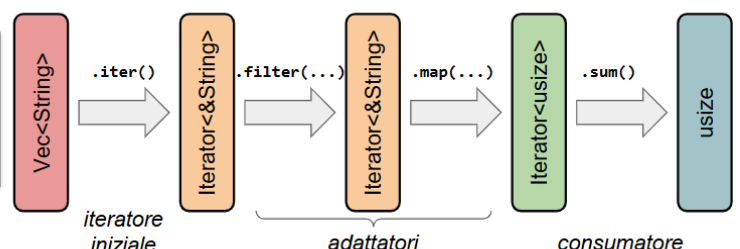
\includegraphics[width=1\linewidth]{content/API_Programming/images/2026-04-03-16-20-34.png}
  \end{minipage}
\end{center}




I principali adattatori:
\begin{itemize}
  \item \mintinline{rust}|map(self, f)|: Esegue la chiusura ricevuta come argomento su ogni elemento dell'iteratore ritornato.
  \item \mintinline{rust}|filter(self, predicate)|: Ritorna un iteratore che restituisce solo gli elementi per i quali l'esecuzione della chiusura ritorna \verb|true|.
  \item \mintinline{rust}|filter_map(self, f)|: Concatena in maniera concisa filter e map; l'iteratore risultante conterrà solo elementi per i quali la chiusura ritorna \verb|Some(B)|.
  \item \mintinline{rust}|flatten(self)|: Ritorna un iteratore dal quale sono state rimosse le strutture annidate.
  \item \mintinline{rust}|flat_map(self, f)|: Concatena map e flatten, esegue la chiusura e rimuove le strutture annidate.
  \item \mintinline{rust}|take(self, n)|: Ritorna un iteratore che contiene al più i primi \verb|n| elementi dell'iteratore su cui viene eseguito.
  \item \mintinline{rust}|take_while(self, predicate)|: Conserva tutti gli elementi fino a quando la funzione ritorna \verb|true|; dal momento in cui diventa \verb|false|, scarta tutti i valori rimanenti.
  \item \mintinline{rust}|skip(self, n)|: Ritorna un iteratore che esclude i primi \verb|n| elementi dell'iteratore originale.
  \item \mintinline{rust}|skip_while(self, predicate)|: Esclude tutti gli elementi fino a quando la funzione ritorna \verb|false|, dal momento in cui diventa \verb|true| conserva tutti i valori rimanenti.
  \item \mintinline{rust}|peekable(self)|: Permette di chiamare i metodi \mintinline{rust}|peek()| e \mintinline{rust}|peek_mut()| per accedere al valore successivo senza consumarlo.
  \item \mintinline{rust}|fuse(self)|: Ritorna un iteratore che termina dopo il primo \verb|None|.
  \item \mintinline{rust}|rev(self)|: Ritorna un iteratore con la direzione invertita.
  \item \mintinline{rust}|inspect(self, f)|: Preleva un elemento dall'iteratore a monte e la passa sia alla funzione (che può ispezionarlo) che al consumatore a valle.
  \item \mintinline{rust}|chain(self, other)|: Prende un iteratore e lo concatena all'originale.
  \item \mintinline{rust}|enumerate(self)|: Ritorna un iteratore che restituisce una tupla formata dall'indice dell'iterazione e dal valore \verb|(i, val)|.
  \item \mintinline{rust}|zip(self, other)|: Combina due iteratori per ritornare le coppie composte dai valori dei primi due iteratori.
  \item \mintinline{rust}|by_ref(&mut self)|: Prende in prestito un iteratore senza consumarlo, lasciando intatto il possesso dell'originale.
  \item \mintinline{rust}|copied(self)| e \mintinline{rust}|cloned(self)|: Ritornano un iteratore dove gli elementi originali vengono, rispettivamente, copiati o clonati.
  \item \mintinline{rust}|cycle(self)|: Raggiunta la fine di un iteratore riparte dall'inizio, ciclando all'infinito.
\end{itemize}


\section{Consumatori}
I consumatori sono i metodi che "finalizzano" la catena dell'iteratore eseguendone l'elaborazione.
\begin{itemize}
  \item \mintinline{rust}|for_each(self, f)|: Esegue la chiusura ricevuta su tutti gli elementi dell'iteratore.
  \item \mintinline{rust}|try_for_each(&mut self, f)|: Esegue una chiusura che può fallire su tutti gli elementi, fermandosi al primo fallimento.
  \item \mintinline{rust}|collect(self)|: Trasforma un iteratore in una collezione.
  \item \mintinline{rust}|nth(&mut self, n)|: Ritorna l'ennesimo elemento dell'iteratore.
  \item \mintinline{rust}|all(&mut self, f)| e \mintinline{rust}|any(&mut self, f)|: Verificano se la chiusura restituisce \verb|true|, rispettivamente, per tutti o per almeno un elemento dell'iteratore.
  \item \mintinline{rust}|find(&mut self, predicate)|: Cerca un elemento sulla base della chiusura ricevuta e lo ritorna.
  \item \mintinline{rust}|count(self)|: Ritorna il numero di elementi dell'iteratore.
  \item \mintinline{rust}|sum(self)| e \mintinline{rust}|product(self)|: Rispettivamente, somma o moltiplica tutti gli elementi di un iteratore e ritorna il valore ottenuto.
  \item \mintinline{rust}|max(self)| e \mintinline{rust}|min(self)|: Ritornano il massimo o il minimo tra gli elementi; se l'iteratore è vuoto ritornano \verb|None|.
  \item \mintinline{rust}|max_by(self, compare)| / \mintinline{rust}|min_by(self, compare)|: Ritornano il massimo o il minimo sulla base della chiusura di confronto ricevuta in argomento.
  \item \mintinline{rust}|max_by_key(self, f)| / \mintinline{rust}|min_by_key(self, f)|: Eseguono la chiusura ricevuta e ritornano l'elemento che produce il risultato massimo o minimo.
  \item \mintinline{rust}|position(&mut self, predicate)| e \mintinline{rust}|rposition(&mut self, predicate)|: Cercano un elemento sulla base della chiusura e ne ritornano la posizione (partendo rispettivamente da sinistra o da destra).
  \item \mintinline{rust}|fold(self, init, f)|: Esegue la chiusura accumulando i risultati sul primo argomento ricevuto (\verb|init|).
  \item \mintinline{rust}|try_fold(&mut self, init, f)|: Come \verb|fold|, ma si ferma al primo fallimento della chiusura.
  \item \mintinline{rust}|last(self)|: Ritorna l'ultimo elemento dell'iteratore.
  \item \mintinline{rust}|find_map(&mut self, f)|: Esegue la chiusura su tutti gli elementi e ritorna il primo risultato valido.
  \item \mintinline{rust}|partition(self, f)|: Consuma un iteratore e ritorna due collezioni sulla base del predicato.
  \item \mintinline{rust}|reduce(self, f)|: Riduce l'iteratore ad un singolo elemento eseguendo la funzione ricevuta.
  \item Confronti tra iteratori: \mintinline{rust}|cmp(self, other)|, \mintinline{rust}|eq(self, other)|, \mintinline{rust}|ne(self, other)|, \mintinline{rust}|lt(self, other)|, \mintinline{rust}|le(self, other)|, \mintinline{rust}|gt(self, other)|, \mintinline{rust}|ge(self, other)|.
\end{itemize}
